\section{논의와 연구 범위}
\label{sec:discussion}

본 장에서는 5장의 결과가 무엇을 뜻하는지, 그리고 그 결과를 어디까지 해석할 수 있는지 설명한다. 핵심은 기본 CoC를 실행 가드로 보완하는 학습과, 실제 실행 단계에서 궤적을 다시 검사하는 일을 구분하는 것이다.

\subsection{기본 CoC와 실행 가드가 맡는 역할}

기본 CoC는 "보행자에게 양보한 뒤 진행한다"처럼 달성할 행동과 그 이유를 설명한다. 실행 가드는 "정지선을 넘지 않는다" 또는 "상충 구역이 1.5초 동안 비어 있을 때만 출발한다"처럼 그 행동을 언제, 어느 범위에서 허용할지를 정한다. Safety-Constrained CoC는 이 두 정보를 한 문맥에 넣은 \textbf{제약 통합 CoC}이며, 영어로만 작성한 표와 그림 내부에서는 \textit{Constraint-integrated CoC (proposed)}로 표시하였다.

표준 시간 과제에서 기본 CoC(제약 없음)의 가드 위반률은 0.319였지만 제약 통합 CoC는 0.000이었다. 이 결과는 기본 CoC가 위험하다는 뜻이 아니다. 기본 CoC에는 짧게 기다릴지 길게 기다릴지를 구분할 정보가 없었고, 동일 입력에 서로 다른 정답이 연결되므로 후보 정확도 0.500과 계약 쌍 정확도 0.000은 구조적으로 예상된다. 실행 가드를 추가하고 올바른 후보와 함께 학습했을 때 모델이 표준 분포에서 그 차이를 배울 수 있었다는 것이 정확한 해석이다. 따라서 본 논문의 기여는 기존 CoC를 부정하는 것이 아니라, CoC가 말하지 않은 허용 조건을 학습 가능한 형태로 보완하고 그 사용 여부를 쌍대 계약으로 측정하는 데 있다.

\revtwo{이 관점에서 제안 방법의 비교 우위는 더 큰 범용 주행 모델을 만드는 데 있지 않다. 행동 목표와 허용조건을 분리해 사람이 읽을 수 있게 하고, 같은 장면의 가드만 바꾸어 조건 사용 여부를 진단하며, 모델 외부 검증으로 위반ㆍ목표 포기ㆍ과도한 보수성을 구별할 수 있다는 데 있다. 표준 시간 평가에서 위반률 0.000, 가드 준수 목표 완료율 1.000 및 계약 쌍 정확도 1.000이 동시에 나타난 것은 이 세 판정이 서로 모순되지 않았음을 보여준다. 다만 미관측 시간값에서 세 지표가 함께 악화되었으므로 이 장점은 현재 합성 표준 분포에서 확인된 진단적 장점으로 한정한다.}

\subsection{제약 통합 CoC가 높은 결과를 보인 이유}

\revone{표준 시간 과제의 position-only ablation에서 제약 통합 CoC와 별도 자연어 제약은 같은 가드 문장ㆍ학습 예ㆍ학습량을 사용했지만 계약 쌍 정확도가 각각 1.000과 0.396이었다. 이는 현재 시간 과제에서 목표와 가드를 한 문맥에 놓는 위치ㆍ구획 방식이 크게 작용했음을 보여주며, 의미 학습만의 효과로 해석할 수 없다. 한편 위치를 별도 필드로 고정하면 올바른 대응과 대응 교란의 계약 쌍 정확도가 0.396과 0.021이므로, 위치 효과와 별개로 올바른 가드--행동 대응도 필요했다. 다만 통합 위치의 대응 교란 조건이 없는 불완전한 요인 설계이고, 정적 과제의 통합/별도 차이는 1.000/0.986으로 작았다. 따라서 현재 증거는 통합 위치의 보편적 우월성이 아니라 과제 의존적 위치 효과와 의미 대응 효과가 모두 존재함을 지지한다. 제약 통합 CoC도 동일 의미 문장 변형 평가에서 계약 쌍 정확도 0.715, 미관측 시간값 평가에서 0.306으로 낮아졌으므로 표준 분포의 높은 성능을 일반적인 시간 추론 능력으로 볼 수 없다.}

그러나 이 결과만으로 자연어가 논리식보다 본질적으로 우수하다고 결론 내릴 수는 없다. 정적 후보 실험에서는 논리식 제약도 위반률 0.000과 계약 쌍 정확도 1.000을 기록하였다. 표현 방식을 공정하게 비교하려면 논리 문법을 따로 학습시키고, 각 조건에 같은 양의 학습 자료와 학습 횟수를 제공한 뒤 다시 평가해야 한다. 현재 결과가 직접 보여주는 것은 자연어의 보편적 우수성이 아니라, 현재 VLM과 학습 조건에서는 제약 통합 CoC가 가장 안정적이었다는 점이다.

\subsection{수치 조건은 모델 외부 검증기가 다시 확인해야 한다}

다중 주행의 복합 표현 변화 평가에서 관찰된 오답 15개는 모두 같은 거리를 m 대신 cm로 표현한 문장에서 발생하였다. 그러나 경계 등호, 부정ㆍ금지, 절 순서 및 단위 변화가 한 평가에 함께 있으므로 단위 변환만을 유일한 원인으로 분리한 결과는 아니다. 더구나 시간 과제의 미관측 시간값 평가에서도 위반률이 0.351로 증가하였다. 모델이 새로운 수치와 단위를 항상 정확하게 처리한다고 볼 수 없으므로, 실제 적용에서는 모델에 모든 계산을 맡기지 않고 그림~\ref{fig:future-architecture}과 같이 역할을 나누는 것이 적절하다.

먼저 모델은 자연어 Safety-Constrained CoC에서 행동 목표와 실행 가드의 의미를 읽는다. 다음 단계에서는 "최소 간격 600 cm"를 조건 종류, 비교 방향, 값과 단위로 나눈다. 그 뒤 600 cm를 6.0 m처럼 기준 단위로 통일한다. 마지막으로 모델 외부 결정적 검증기 또는 차단장치가 선택한 궤적의 거리, 속도와 시간 조건을 수치로 검사한다.

\revone{저장 어댑터의 재평가는 이 구조의 실용적 이점과 한계를 함께 보여준다. cm 경계만 동등한 m 값으로 바꾸자 세 건의 안전하지 않은 선택이 모두 교정되어 가드 위반률은 0.010에서 0.000으로 낮아졌지만, 후보 정확도와 계약 쌍 정확도의 향상은 각각 0.010과 0.021에 그쳤다. 남은 12건은 모두 안전하지만 과도하게 보수적인 차선 변경 선택이었다. \revfinal{즉 이 복합 표현 조건에서는 결정적 단위 정규화가 수치 위반을 줄였지만, 남은 오류가 부정 표현ㆍ절 순서ㆍ경계 등호 중 어느 요인 또는 그 상호작용에서 비롯되었는지는 분리하여 확인하지 못했다.}}

이 과정에서는 "미만"과 "이하"처럼 경계값 포함 여부를 구분해야 한다. 또한 가드를 지킬 수 없을 때 정지할지, 다시 기다릴지와 같은 대체 행동도 정해야 한다. 모델은 문장의 목표와 조건을 해석하고, 검증기는 정확한 수치 경계를 확인하도록 역할을 나누는 것이다.

\begin{figure}[t]
\centering
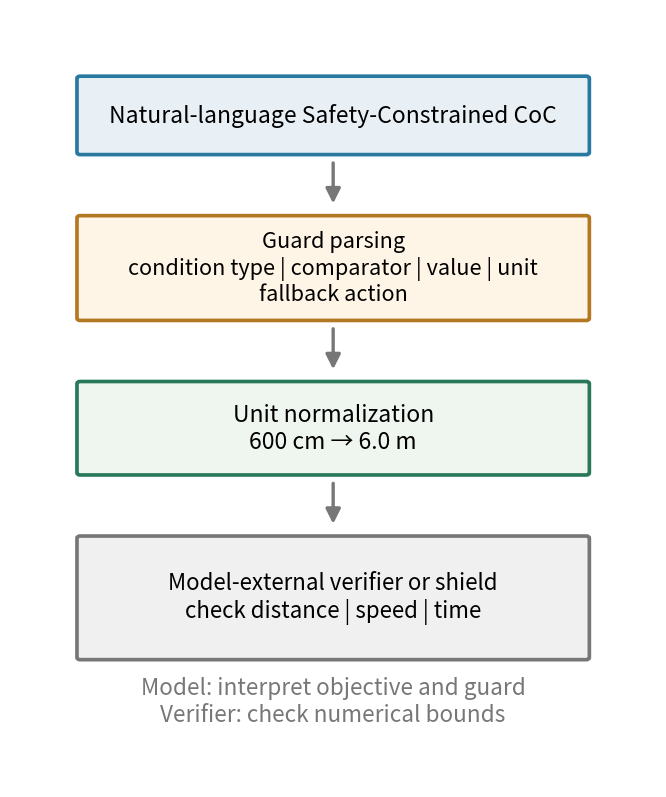
\includegraphics[width=0.94\columnwidth,trim=18 22 18 22,clip]{../latex-kiee-review-2022/figures/fig05_typed_contract.png}
\bifigcaption{자연어 실행 가드를 실제 검사에 연결하는 네 단계. 위에서 아래로 (1) 자연어 제약 통합 CoC를 읽고, (2) 조건 종류ㆍ비교 방향ㆍ값ㆍ단위ㆍ대체 행동으로 나누며, (3) 600 cm를 6.0 m처럼 기준 단위로 통일하고, (4) 모델 외부 검증기 또는 차단장치가 선택한 궤적의 거리ㆍ속도ㆍ시간을 수치 경계와 비교한다. 모델은 목표와 가드를 해석하고 결정적 검증기는 정확한 수치 판정을 담당한다.}{Four-stage path from a natural-language execution guard to typed fields, unit normalization, and deterministic runtime verification.}
\label{fig:future-architecture}
\end{figure}

\subsection{학습된 가드와 실행 차단장치는 역할이 다르다}

가드를 학습하면 모델이 가드를 지키는 후보를 선택할 가능성이 높아진다. 그러나 학습에서 보지 못한 모든 상황에서 준수를 보장하지는 않는다. 폐루프의 해제 후 재위험 상황에서 동적 계약은 가드 위반률을 46.6\%에서 21.4\%로 줄였지만 위반을 없애지는 못했다. 최신 상태를 사용하는 차단장치를 함께 적용했을 때 위반률은 4.8\%까지 낮아졌다. 이는 학습된 계약과 실행 단계 검사가 서로 다른 역할을 맡는다는 것을 보여준다.

차단장치도 모든 문제를 해결하지는 못한다. 계약 정보가 0.4초 늦게 도착했을 때 계약+차단장치의 위반률은 34.8\%로 증가하였다. 계약 자체가 틀리거나 중요한 위험이 빠져 있어도 차단장치는 잘못된 조건을 정확하게 집행할 뿐이다. 따라서 실제 시스템에서는 위험이 다시 나타나면 출발 허용을 취소하고 대기 상태로 돌아갈 수 있어야 한다. 계약이 어느 시점의 상황을 설명하는지도 확인해야 하며, 미래 상황이 불확실하면 더 신중한 대체 행동을 선택해야 한다.

\revone{동적 계약과 단조 단계 계약의 차이는 이 갱신 요구를 직접 드러낸다. 출발 허용은 영구적인 단계 완료가 아니라 현재 관측에 의존하는 임시 허가이므로, 위험이 재등장하면 계약 상태도 $\mathrm{RELEASED}$에서 $\mathrm{HOLD}$로 되돌아가야 한다. 이 역전이를 허용한 동적 계약은 단조 단계 계약보다 위반률을 16.5\%p, 충돌률을 11.6\%p 낮췄다. 반대로 계약 갱신이 0.4초 늦어지면 동적 계약의 위반률이 48.1\%로 악화된 결과는 상태의 가역성뿐 아니라 최신성도 필요함을 보여준다. 이 결과는 별도 소형 폐루프 환경의 메커니즘 증거이며 실제 차량에서 같은 감소폭을 보장하지 않는다.}

\revone{또한 표~\ref{tab:shield-cost}은 차단장치의 가치를 안전 이득과 비용으로 함께 판단해야 함을 보여준다. 해제 후 재위험에서는 위반ㆍ충돌 감소가 있었지만 episode당 9.935회 개입과 가가속도 증가가 동반되었다. 반대로 phase-complete bank에서는 1.269--2.539회 개입하고 진행거리와 가가속도가 소폭 악화되었지만 추가적인 이진 안전 이득은 없었다. 그러므로 차단장치는 상시적인 무비용 보장 장치가 아니라, 학습 정책의 잔여 위험과 개입 비용을 함께 측정하여 적용 범위를 정해야 하는 구성요소다.}

\subsection{주 실험이 실제로 확인한 것}

주 실험은 모델이 연속 궤적을 새로 생성하는 문제가 아니다. 합성 이미지와 수치가 적힌 궤적 후보를 주고 그중 하나를 선택하게 한 실험이다. 따라서 이 실험이 직접 확인한 것은 모델 입력에 포함된 실행 가드가 후보 선택에 조건으로 사용될 수 있는가이다. 입력 형식을 맞춘 비교에서 올바른 대응 학습의 계약 쌍 정확도가 제약--정답 대응 교란보다 높았다는 결과가 이 주장을 가장 직접적으로 뒷받침한다. 정적ㆍ시간 과제에서는 별도 자연어 제약과 대응 교란을, 다중 주행 과제에서는 제약 통합 CoC와 대응 교란을 비교해야 한다. 입력 형식이 다른 조건의 차이를 올바른 대응 관계만의 효과로 해석하지 않는다.

쌍대 계약은 같은 장면에서 가드만 바꾸므로 장면만 보고 같은 답을 반복하는 방법을 막는다. 가드 준수 목표 완료율은 모델이 가드 위반을 피하려고 끝까지 정지하는 방법도 막는다. 이 두 지표를 함께 사용하면 모델이 행동 목표를 끝내면서 가드에 맞는 후보를 골랐는지 확인할 수 있다. 영상 절제에서는 표준 시간 과제의 후보 정확도가 원본 1.000에서 단색 영상 0.670과 `상충 구역이 비기 시작한 시각'이 실제와 다른 충돌 영상 0.608로 낮아져 합성 연속 장면 영상의 시간 정보 사용이 확인되었다. 그러나 다중 주행의 표준ㆍ미관측 수치 평가는 단색 및 반대 행동 영상에서도 1.000을 유지하였다. 즉 영상 의존성은 과제별로 달랐고, 다중 주행의 높은 점수는 문장에 적힌 행동 종류와 후보 수치만으로 설명된다. 시간 과제도 글자가 그려진 합성 연속 장면 영상이므로 실제 센서 장면의 시각적 근거화로 일반화할 수 없다. 후보의 물리량, 정답과 검증 규칙도 같은 합성 과제에서 설계되었으므로 모델 외부 검증기는 외부 안전 정답이 아니다. 그러므로 높은 점수는 제한된 후보 선택 문제에서의 가드 학습 효과이지 실제 차량 안전의 증명이 아니다.

Alpamayo-R1 진단, Qwen 후보 선택 및 소형 신경망 폐루프 실험도 증거의 역할이 다르다. 단일 장면 Alpamayo-R1 결과는 입력 문장에 대한 민감도 진단이고, Qwen 결과가 제안 표현의 중심 학습 증거이며, 폐루프 미시 환경은 최신 계약과 차단장치의 필요성을 예시한다. 따라서 세 결과를 같은 모델에서 단계적으로 안전성이 향상되었다는 하나의 인과 사슬로 합칠 수 없다.

\subsection{결과를 해석할 때의 실험적 한계}

후보 문자를 장면마다 바꾸어 같은 문자만 고르는 암기를 막았고, 제약--정답 대응 교란 통제군으로 문장 추가 자체의 효과를 구분하였다. 시간 및 다중 주행 과제는 세 난수 초기값으로 반복했으며, 각 초기값은 학습 난수뿐 아니라 합성 장면 값과 후보 문자 배치도 바꾼다. 이러한 설계는 전체 실험 절차의 반복성을 확인하지만, 동일 데이터를 고정한 최적화 분산만을 추정하지는 않는다.

다만 반복 횟수가 세 번으로 적고, 정적 후보 결과는 한 난수 초기값만 사용하였다. \revfinal{시간 표와 다중 주행 표는 기존 집계 구현과의 대응을 유지하여 각각 모집단ㆍ표본 표준편차를 보고한다. 두 정의의 차이와 해석 범위는 5장 도입부에 명시했으며, 과제 간 표준편차의 크기를 직접 비교하지 않는다.} 영상 절제는 저장 어댑터의 추론을 반복했으므로 새로운 학습 반복을 추가하거나 자연 영상 분포를 시험한 결과가 아니다. 충돌 영상은 모델이 보아야 할 문제 전제 자체를 바꾸므로, 그 조건에서 우연히 낮아진 위반률은 강건성 개선으로 해석할 수 없다. 복합 표현 변화 평가에는 단위 변환, 부정 표현, 경계값과 조건 순서 변경이 함께 들어 있다. \revfinal{오답이 cm 문장에 집중되었지만, 현재 결과만으로 특정 요인을 성능 저하의 주된 원인으로 지목하거나 요인별 기여도를 추정할 수는 없다.} 후속 실험에서는 장면과 나머지 문장을 고정하고 단위, 부정 표현, 경계값 포함 여부와 복합 조건을 한 번에 하나씩만 바꾸어 각 요인의 영향을 분리해야 한다.

\revone{\revfinal{표준 평가는 학습과 같은 문장 틀ㆍ수치 범위에서 제한된 후보를 선택하는 과제이므로, 일부 정확도 1.000에는 이러한 난이도와 제한된 평가 범위에 따른 천장 효과(ceiling effect)가 반영되었을 가능성이 있다. 따라서 1.000은 해당 표준 분포에서의 가드 조건화 학습을 보여주지만, 일반적인 수치 추론 능력이나 더 어려운 조건에서의 성능을 입증하지 않는다. 표~\ref{tab:maneuver}의 hard-case에서는 계약 쌍 정확도가 정지 0.958, 차선 변경 0.833으로 낮아졌다. 표준 결과는 이 hard-case 결과와 함께 해석해야 하며, hard-case에서도 동시 제약ㆍ경계 등호ㆍ표현 변화가 결합되어 있으므로 하락을 특정 난이도 요인 하나의 효과로 단정할 수 없다. 후속 평가에서는 가드 간 수치 간격과 활성 제약 수 등을 독립적으로 변화시켜 난이도의 영향을 분리할 필요가 있다.}}

\subsection{실제 제약 조건의 생성은 본 논문의 범위가 아니다}

본 논문은 주어진 실행 가드를 CoC와 결합했을 때 모델의 궤적 선택이 달라지는지를 평가한다. 그러나 실제 주행 장면에서 어떤 가드가 필요한지 발견하고, 최소 간격이나 제한 시간의 값을 정하며, 위험이 해소되었다고 판단할 해제 조건을 생성하는 방법은 제안하지 않았다. 실험의 가드는 연구자가 합성 과제의 정답이 분명하도록 미리 설정한 것으로, 교통 법규, 운행설계영역(ODD), 차량 동역학 또는 안전 분석에서 도출한 실제 차량 요구사항이 아니다. 따라서 높은 가드 준수율은 이미 주어진 조건을 모델이 학습하고 적용할 수 있음을 뜻할 뿐, 그 조건 자체가 충분하거나 안전하게 생성되었음을 뜻하지 않는다.

실제 제약 조건을 개발하려면 먼저 CoC가 설명하는 객체, 원인, 요구 행동과 시간 순서를 추출하고, 이를 교통 법규, 시스템 안전 요구사항, ODD, 차량의 제동ㆍ조향 한계 및 센서 불확실성과 연결해야 한다. 다음으로 각 근거를 조건 종류, 적용 대상, 비교 방향, 값ㆍ단위, 유지 구간, 해제 조건 및 불확실성 대체 행동을 포함한 구조화 가드로 변환해야 한다. 이렇게 얻은 후보 가드는 도메인 전문가의 검토와 출처 추적을 거친 뒤, 시뮬레이션과 반례 탐색에서 지나치게 느슨하거나 보수적인 조건을 찾아 반복 수정해야 한다. 이 과정은 본 논문의 학습 및 평가 방법보다 앞선 별도의 요구사항 공학 문제이다.

\subsection{Alpamayo-R1과 실제 도로로 확장할 때의 범위}

작은 Qwen VLM의 후보 선택 결과가 Alpamayo-R1의 연속 궤적 생성에서도 그대로 나타난다고 볼 수는 없다. Alpamayo-R1 사전 진단은 한 장면에서 CoC에 추가된 문장에 대한 궤적 변화가 반대 의미 사이의 변화보다 컸다는 관찰만 제공한다. Alpamayo-R1에도 같은 효과가 있는지 확인하려면 가드 준수 학습을 직접 수행한 뒤 연속 궤적을 별도 기준으로 검증해야 한다.

또한 본 논문의 실행 가드는 도로 안전 전체가 아니라 정지선, 최소 간격, 속도와 대기시간 같은 일부 조건만 다룬다. 실제 도로에서는 센서에 보행자나 차량이 실제로 보이는지, 보행자·자전거·차량의 위치와 이동 경로가 어떻게 겹치는지, 선택한 궤적의 충돌 위험은 얼마인지도 확인해야 한다. 계약이 센서의 어느 시점과 대응하는지 기록하고, 사람의 검토나 측정값으로 만든 독립된 정답 자료와 비교하는 평가도 필요하다. 따라서 다음 단계는 작은 VLM 결과를 실제 안전으로 확대 해석하는 것이 아니라, Alpamayo-R1의 연속 궤적과 실제 센서 근거에서 같은 질문을 다시 검증하는 것이다.
